
\documentclass[12pt]{article}
\usepackage[a4paper, margin=.30in]{geometry}
\usepackage{graphicx ,
            wrapfig,
            xcolor, 
            enumerate,
            amsmath,
			fontenc,
			tcolorbox,circuitikz,tikz,bm
            }
			\usepackage{pgfplots}
\pgfplotsset{compat=newest}
\usepgfplotslibrary{fillbetween}
%\usepackage{scalerel}
%\usepackage{pict2e}
%\usepackage{tkz-euclide}
%\usetikzlibrary{calc}
%\usetikzlibrary{patterns,arrows.meta}
%\usetikzlibrary{shadows}
%\usetikzlibrary{external}

%%pgfplots
\usepackage{pgfplots}
%\pgfplotsset{compat=newest}
%\usepgfplotslibrary{statistics}
%\usepgfplotslibrary{fillbetween}

\newcommand\headerMe[2]{\noindent{}#1\hfill#2}
\renewcommand{\thesection}{\Roman{section}}

\author{Zakaria HAOUZAN}
\date{\today}

\begin{document}
% headers --------------
\headerMe{Matière : Physique-Chimie}{Professeur : Zakaria HAOUZAN}\\
\headerMe{Unité : Mécanique }{Établissement : Lycée SKHOR qualifiant}\\
\headerMe{Niveau : 2BAC-SM-PC}{Heure : 7H}\\

% ------Content ________
\begin{center}

    \Large{Leçon $N^{\circ} 12 $: \color{red} Les mouvement plans}
\end{center}

%\begin{wrapfigure}[10]{r}{0.5\textwidth}
%    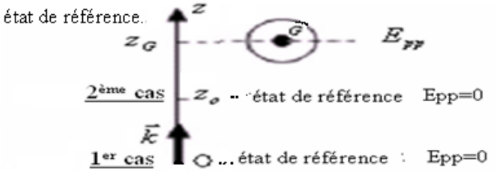
\includegraphics[width=0.5\textwidth]{./img/img00.png}
%\end{wrapfigure}

\section{Le mouvement d'un projectile dans le champ de pesanteur:}

\subsection{Trajectoire du projectile : }

Tous corps immergé dans un fluide est soumis à trois forces :  


Au début la bille est maintenue par électroaimant puis lâchée du haut d’un rail ,elle roule le long du rail et elle le
quitte avec une vitesse initiale horizontale puis elle tombe sur une plaque horizontale.
En faisant varier la position de la plaque et en indiquant chaque fois sa position de chute de la bille, on obtient la
trajetoire de son mouvement: c'est une trajetoire parabolique.

\subsection{Etude du mouvement du projectile :}

Un projectile de masse m est lancé d'un point O à l'instant $t=0$ avec une vitesse $\vec{v_0}$ qui fait un angle $\alpha$ avec l'horizontale.

On considère un repère $(O, \vec{i}, \vec{j})$ confondu avec le plan du mouvement du projectile et qu'on suppose galiléen.

\begin{itemize}
	\item Le système étudié :{le projectile}
	\item Bilan des forces: le projectile est soumis uniquement à l'action de son poids :
		(Le projectile a une grande densité ,donc la poussée d'Archimède et les forces de frottement fluides sont négligeable)
	\item Les conditions initiales à $t=0$ ,$x_0=0$ et $y_0=0$
	\item Les coordonées du vecteur vitesse initiale sont : 
		$\begin{cases} v_{0x} = v_0.cos(\alpha)\\v_{0y} = v_0.sin(\alpha)
\end{cases}$
	\item En appliquant la 2ème loi de Newton : $\sum \vec{F}=m\vec{a_G}$ donc $\vec{P} = m.\vec{a_G}$ (1)

	\item  Par projection de la relation (1) dans le repère (O,x,y): 
$\begin{cases}P_x = m.a_x\\P_y = m.a_y\end{cases}$
 alors $\begin{cases}0 = m.a_x\\-P = m.a_y\end{cases}$
 donc $\begin{cases}a_x = 0\\a_y = -g\end{cases}$
 avec $\begin{cases}\frac{dv_x}{dt} = 0\\\frac{dv_y}{dt} = -g\end{cases}$  $\rightarrow$ 
  $\begin{cases}v_x = C\\v_y = -gt+C'\end{cases}$

\item On détermine les constantes C et C' d'après les conditions initiales : à t=0 : 

	$\begin{cases} v_{0x} = v_0.cos(\alpha)\\v_{0y} = v_0.sin(\alpha) \end{cases}  \Rightarrow$ 	
	$\begin{cases} v_{x} = v_0.cos(\alpha)\\v_{y} = -g.t +v_0.sin(\alpha) \end{cases} $
	d’où  $\begin{cases} \frac{dx}{dt} = v_0.cos(\alpha)\\\frac{dy}{dt} = -gt+v_0.sin(\alpha) \end{cases}$ 	

	donc  : $\begin{cases} x = v_0.cos(\alpha).t + K\\y = \frac{-1}{2}.gt^2 + v_0.sin(\alpha).t + K' \end{cases}$ 	

\item On détermine les constantes K et K' d'après les conditions initiales : à t=0 , xo=0 et yo=0 donc :K=0 et K'=0. 
	 
	Et on obtient les équations horaires du mouvement du projectile : $\begin{cases} x = v_0.cos(\alpha).t + K\\y = \frac{-1}{2}.gt^2 + v_0.sin(\alpha).t + K' \end{cases}$


	\item On obtient l'équation de la trajectoire en éliminant t entre x et y.

	On a $t =  \frac{x}{v_0.cos(\alpha)}$ en remplaçant dans y : $y = -\frac{g}{2.v_0^2.cos(\alpha)^2}.x^2 +xtan(\alpha)$

\item Le sommet S de la trajectoire : c'est le plus haut point atteint par le projectile au cours de son mouvement.
	\begin{itemize}
		\item Au sommet de la trajectoire on a $v_y = 0$ donc $t=\frac{v_0.sin(\alpha)}{g}$
		\item Et en remplaçant dans x et y on obtient les coordonnées du sommet S de la trajectoire du projectile. $y_s =\frac{v_0^2.sin(\alpha)^2}{2g}$ et $x_s = \frac{v_0^2.sin(2.\alpha)}{2g}$
		\item avec: $sin(2\alpha) =2.sin(\alpha) . cos(\alpha)$
	\end{itemize}

\item La portée :c'est la distance OP qui sépare le point de lancement du projectile et le point de sa tombée sur ox. Au point P on a $y_p = 0 \Rightarrow 0 = -\frac{g}{2.v_0^2.cos(\alpha)^2}.x^2 +xtan(\alpha)$alors : $\begin{cases} x_p = 0 \\ x_p = \frac{x^2.sin(2\alpha)}{g}\end{cases}$
\item Remarque: La plus grande portée correspond à $sin(2.\alpha) =1$ donc $\alpha = \frac{\pi}{4}$

\end{itemize}








---------------------------------------------------------------------------
\begin{itemize}
	\item $\vec{P}$ : La force de pesanteur (poids du corps)
	\item $\vec{F_A}$: la poussée d'archimède.
	\item $\vec{f}$ : La force de frottement fluide exercée par le fluide. 
\end{itemize}

\subsection{La force de pesanteur: }
Dans le champ de pesanteur, au voisinage de la terre, les corps son soumis à une force de pesanteur exercée par la terre qui s'appelle : poids du corps.

\begin{itemize}
	\item Relation entre poids et masse d’un corps : $P = m.g$
		\item la force: $\vec{P} = m.\vec{g}$ s'applique au centre d'inertie du corps.

		\item g : Intensité du champ de pesanteur (en $ N/kg)$ ou $(m/s^2)$.

\end{itemize}
\subsection{La poussée d'Archimède:}
Tout corps immergé totalement ou partiellement dans un fluide est soumis à une force exercée par ce fluide qui
s'appelle la poussée d'Archimède ,sa direction est toujours verticale orientée vers le haut d'intensité égale au poids
du liquide déplacée : $F_A = m_f.g$ avec $m_f = \rho_f.V$

Expression de la poussée d‘Archimède : $\vec{F_A} = - \rho_f.V.\vec{g}$ elle s'applique au centre d'inertie du corps.

- $\rho_f$ : la masse volumique du fluide en $(kg/m^3)$

- V :  volume du liquide déplacé en $(m^3)$

- g : intensité de pesanteur en $(N/kg)$ ou $(m/s^2)$

\subsection{La force de frottement fluide:}
Les forces de frottements exercées par un fluide sur un corps immergé dedans sont équivalente à une force unique $\vec{f}$ appelée force de frottement fluide $\vec{f} = -k.\vec{v^n}$ de direction opposée à la vitesse et d'intensité: $f = k.v^n$

\begin{itemize}
	\item Si la vitesse est faible on prend n=1 et la force de frottement devient : $f = k.v$
	\item Si la vitesse est grande on prend n=2 et la force de frottement devient : $f = k.v^2$
\end{itemize}

\section{La chute verticale d'un corps dans un fluide par frottement :} 
\subsection{Equation différentielle vérifiée par la vitesse :  }

\begin{wrapfigure}[1]{r}{0.2\textwidth}
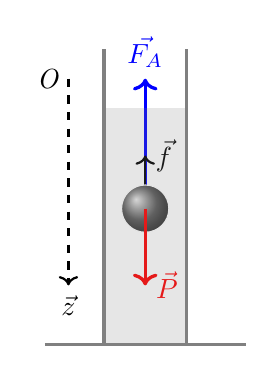
\begin{tikzpicture}[scale=0.75, decoration={coil,aspect=0.4,segment length=3mm,amplitude=3mm}]

	\draw [->, thick, dashed] (4,0.5)node[left]{$\emph{O}$}--(4,-3)node[below ]{$\vec{z}$};
	\draw [<-,very thick, blue] (5.3,0.5)node[above]{$\vec{F_A}$}--(5.3,-1.9);
	\draw [<-,black ,thick] (5.3,-0.8)node[right]{$\vec{f}$}--(5.3,-1.9);
\draw [color=white,ball color=gray,smooth] (5.3,-1.7) circle (0.4) ;
\draw [->,very thick, red] (5.3,-1.7)--(5.3,-3) node[ right]{$\vec{P}$};
%eprouvette rempli de solution
\draw [gray, very thick] (4.6,-4) --++ (0,5);
\draw [gray, very thick] (6.0,-4) --++ (0,5);
\draw [gray, very thick] (3.6,-4) --++ (3.4,0);
\fill [gray,opacity=0.2] (4.6,-4) rectangle (6.0,0);
%fin eprouvette
\end{tikzpicture}
\end{wrapfigure}

Considérons une boule de masse m complétement immergé dans un fluide .

\begin{itemize}
	\item Le système étudié : {La boule }
	\item Choix du repère : On Considèrons le repère (O,z) orienté vers le bas.
	\item Bilan des forces : la boule est soumis à l'action des forces suivantes : 

		\begin{itemize}
			\item $\vec{P}$: son poids $\vec{P} =m.g.\vec{k}$ d'intensité: P=mg
			\item $\vec{F_A}$ : La poussée d'Archimède $\vec{F_A} = -\rho_f.V.g.\vec{k}$ d'intensité: $F_A=\rho_f.V.g$ 
			\item $\vec{f}$: la force de frottement $\vec{f} =-k.v^n.\vec{k}$ d'intensité: $f=k.v^n$

		\end{itemize}
	\item Applications de la deuxième loi de NewTon: $\sum \vec{F_{ext}} = m.\vec{a_G}$ 
		
		donc : $\vec{P} + \vec{F_A} + \vec{f} = m.\vec{a_G}$

	\item En projetant la relation sur l'axe (Oz) : $P-F_A-f = m.a_z$ 

		donc $m.g - m_f.g - K.v^n = m.\frac{dv}{dt}$  avec $m_f = \rho_f.V$
	\item Equation différentielle : $\frac{dv}{dt} = g(1- \frac{m_f}{m} - \frac{k.v^n}{m})$
	Equation différentielle qui est de forme $\frac{dv}{dt} = A- B.v^n$

\end{itemize}

\subsection{Les grandeurs caractérisant le mouvement:}
L'étude expérimentale permet de tracer la courbe de variation de la vitesse de la bille en fonction du temps:
\begin{center}

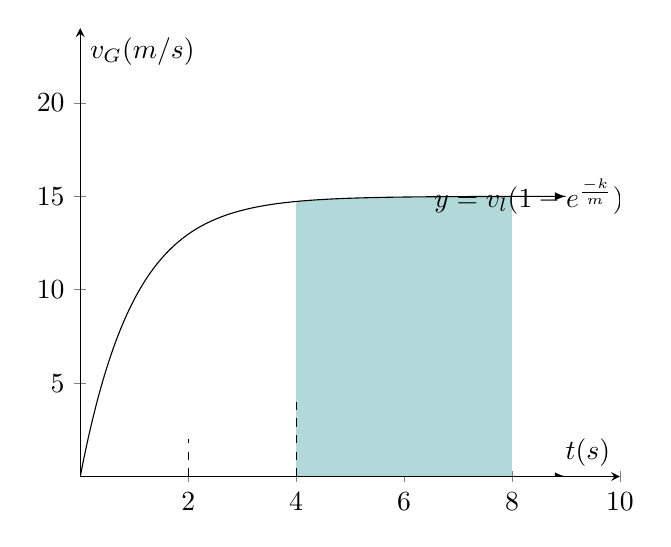
\begin{tikzpicture}
\begin{axis}[
    axis lines = middle,
    xlabel = {$t(s)$},
    ylabel = {$v_G(m/s)$},
    xmin=0, xmax=10,
    ymin=0, ymax=24]
 
% Plot 1
\addplot [name path = A,
    -latex,
    domain = 0:9,
    samples = 1000] {15*(1-e^(-x)) } 
	node [very near end, right] {$y=v_l(1-e^{\frac{-k}{m}})$};
 
% Plot 2
\addplot [name path = B,
    -latex,
    domain = 0:9] {0} 
    node [pos=1, above] {};
 
% Fill area between paths
\addplot [teal!30] fill between [of = A and B, soft clip={domain=4:8}];
 
% Dashed lines
%\draw [dashed, teal] (axis cs:{2,2}) -- (axis cs:{2,4});
%\draw [dashed, teal] (axis cs:{4,4}) -- (axis cs:{4,16});
\draw [dashed] (axis cs:{2,0}) -- (axis cs:{2,2});
\draw [dashed] (axis cs:{4,0}) -- (axis cs:{4,4});
 
\end{axis}
\end{tikzpicture}
\end{center}	
La courbe présente deux régimes:
\begin{itemize}
\item Un régime intial durant lequel:
	\begin{itemize}
		\item La vitesse de la bille augmente.
		\item  La valeur f de la force de frottement du fluide augmente.
		\item  L'accélération de la bille diminue.
	\end{itemize}
\item  Un régime permanent durant lequel:
	\begin{itemize}
		\item La vitesse de la bille devient constante et prend une valeur limite $v_l$
		\item La valeur f de la force de frottement fluide est constante.
		\item L'accélération de la bille est nulle.
	\end{itemize}

\item Or à chaque instant durant le mouvement: $a = \frac{dv}{dt} = g(1 - \frac{m_f}{m}) - \frac{k}{m}.v^n$ 
\item donc l'accélération initiale du mouvement de la bille à $t=0$:  $a_0 = \frac{dv}{dt} = g(1 - \frac{m_f}{m})$
\item $a_0 = \frac{\Delta{v}}{\Delta{t}} = \frac{v_{lim - 0}}{\tau - 0} = \frac{v_{lim}}{\tau}$
\end{itemize}

\section*{-Accélération du mouvement de la bille pendant le régime transitoire :}
Au début du mouvement, la vitesse (de chute de la bille) augmente et son mouvement devient accéléré , son accélération
: donc son accélération diminue au fur et à mesure que sa vitesse augmente.

-La vitesse limite de la bille: $a = \frac{dv}{dt} = g(1 - \frac{m_f}{m}) - \frac{k}{m}.v^n = A- B.v^n$ 

Lorsque le régime permanent est établit la vitesse de la bille devient constante, donc: $\frac{dv}{dt} = 0$

donc , $A-B.v^n = 0$, L’expression de la vitesse limite: $v_l = (\frac{A}{B})^{\frac{1}{n}}$

$$v_l = [\frac{g}{k}(m - m_f)]^{\frac{1}{n}} = [\frac{g}{k}(\rho - \rho_f).V]^{\frac{1}{n}}$$

$\rho $: masse volumique du corps en $(kg/m^3)$

$\rho$ : masse volumique du fluide en $(kg/m^3)$

\begin{tcolorbox}

Remarque: Graphiquement la valeur de l'accélération initiale est égale au coefficient directeur de la tangente à la
courbe v=f(t) à t=0.
\end{tcolorbox}


\section*{-Le temps caractéristique du mouvement:}
Graphiquement l'asymptote à la courbe et la tangente à t=0 se coupent à $t = \tau$
temps caractéristique du mouvement qui est donné par la relation: $v_{lim} = a_0.\tau$

\begin{tcolorbox}
Remarque : Si on connait le temps caractéristique du mouvement on peut évaluer la durée du mouvement initial . car il est égal à environ $5\tau$
\end{tcolorbox}

\subsection{Solution de l'équation différntielle par la méthode d'Euler:}

La méthode d'Euler est une méthode itérative (c'est à dire qu'elle nécessite la répétition d'un même calcul),elle permet de
savoir la vitesse de la bille à instant donné.
Cette méthode comporte deux étapes de calcul.
\section*{La 1ère étape:}

Si on connait la vitesse initiale $v_0$ ,on détermine la valeur de l'accélération initiale $a_0$ à partir de la relation : $a_0 = A-B.v^n_0$.

\section*{La 2ème étape:}
Si on connait le pas de calcul: $\Delta{t} = t_{i+1} - t_i$,on détermine la vitesse $v_{i+1}$ à l'instant $t_{i+1}$ par la relation suivante: $$v_{i+1} = v_i + a_i.\Delta{t}$$

Donc les deux relations intéressantes dans la méthode d'Euler sont : 

 $a_i = A-B.v^n_i$.  et $v_{i+1} = v_i + a_i.\Delta{t}$


 Initialement on connait la valeur de la vitesse initiale $v_0$ : 

 On détermine alors :  $a_0 = A-B.v^n_0$.  puis on en déduit $v_{1} = v_0 + a_0.\Delta{t}$
 
 Et On détermine  :  $a_1 = A-B.v^n_1$.  puis on en déduit $v_{2} = v_1 + a_1.\Delta{t}$
 
 On détermine alors :  $a_2 = A-B.v^n_2$.  puis on en déduit $v_{3} = v_2 + a_2.\Delta{t}$

 ...........et ainsi de suite......


 \begin{tcolorbox}
Remarque :
Le choix du pas du calcul a une grande importance dans la méthode d'Euler, car plus que sa valeur est petite plus
les résultats théoriques sont proches des résultats expérimentaux .

On prend généralement pour pas de calcul $\Delta{t} = \frac{\tau}{10}$ pour ne pas dépasser la vitesse limite de la bille.

 \end{tcolorbox}

 \section{La chute libre d'un corps dans un fluide sans frottement}
 \subsection{Définition de la chute libre:}

\begin{wrapfigure}[1]{r}{0.2\textwidth}
	\vspace{-2cm}
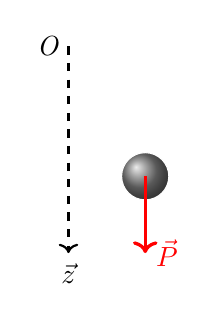
\begin{tikzpicture}[scale=0.75, decoration={coil,aspect=0.4,segment length=3mm,amplitude=3mm}]

	\draw [->, thick, dashed] (4,0.5)node[left]{$\emph{O}$}--(4,-3)node[below ]{$\vec{z}$};
	%\draw [<-,very thick, blue] (5.3,0.5)node[above]{$\vec{F_A}$}--(5.3,-1.9);
	%\draw [<-,black ,thick] (5.3,-0.8)node[right]{$\vec{f}$}--(5.3,-1.9);
\draw [color=white,ball color=gray,smooth] (5.3,-1.7) circle (0.4) ;
\draw [->,very thick, red] (5.3,-1.7)--(5.3,-3) node[ right]{$\vec{P}$};
%eprouvette rempli de solution
%\draw [gray, very thick] (4.6,-4) --++ (0,5);
%\draw [gray, very thick] (6.0,-4) --++ (0,5);
%\draw [gray, very thick] (3.6,-4) --++ (3.4,0);
%%\fill [gray,opacity=0.2] (4.6,-4) rectangle (6.0,0);
%fin eprouvette
\end{tikzpicture}
\end{wrapfigure}


Un corps est en chute libre s'il n'est soumis qu'à l'action de son poids.
Lorsque la trajectoire du corps en chute libre est rectiligne on dit que le corps est en chute 

libre verticale.

Remarque: Pratiquement on peut négliger l'action de l'air sur les corps solides 

denses et ayant une forme aérodynamique

\subsection{Etude de la chute libre d'un corps:}


-Système étudié {la boule}

-Bilan des forces : La boule en chute est soumise uniquement à l'action de son poids

-Choix du référentiel: on considère un repère (O,z) orienté dans le sens du mouvement (voir figure précédente).

- Représentation des forces:

-Application de la 2ème loi de Newton: $\sum \vec{F} = m.\vec{a_G}$ donc $\vec{P} = m.\vec{a_G}$

-En projetant la relation (1) sur (o,z) on a; $P=m.a_z$ donc $a_z=g$

Donc le mouvement de chute libre de la bille est rectiligne uniformément varié :

\begin{itemize}
	\item Son accélération $a_G = g$.
	\item L'équation de la vitesse : $V_G = g.t+v_0$
	\item L'équation horaire du mouvement : $z_G = \frac{1}{2}.g.t^2 + v_0.t + z_0$ 
	\item Pour $v_0 = 0$ et $z_0 = 0$ : $z_G = \frac{1}{2}.g.t^2$ 
\end{itemize}

%wfg---------------------------------------------------------------sf 
%\begin{center}
   %\begin{tabular}{ |c|c|c|c|c|c|c| }
      %\hline
      %km & hm & dam & \bf{m} & dm & cm & mm \\
      %\hline
        %&   &    &  &   &   & \\
%\hline
%\end{tabular}
%On place un seul nombre dans chaque case.
%\end{center}
%\begin{center}
   %\begin{tabular}{ |c|c|c|c|c|c|c| }
      %\hline
      %$km^2$ & $hm^2$ & $dam^2$ & \bf{$m^2$} & $dm^2$ & $cm^2$ & $mm^2$ \\
      %\hline
        %&   &    &  &   &   & \\
%\hline
%\end{tabular}
%\end{center}


\end{document}

